\subsection{\large{Архитектура сервиса запуска расчётных задач}}
\addcontentsline{toc}{subsection}



Для расчёта генерального плана площадного объекта в автоматическом режиме используются четыре типа сущностей,
представленные на диаграмме ниже(см. рис.\ref{pic:architecture__orchestrator-classes})
\begin{figure}[H]
	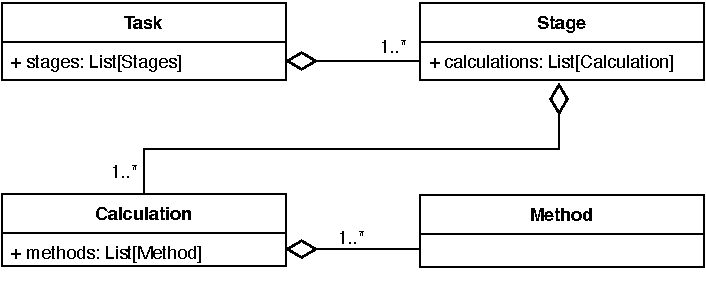
\includegraphics[width=\textwidth]{architecture/pictures/orchestrator/classes}
	\caption{Диаграмма классов}
	\label{pic:architecture__orchestrator-classes-1}
\end{figure}
\vskip 5 mm

\begin{itemize}
	\item {
		\textit{Task} -- расчётная задача. Задача состоит из набора этапов, выполняющихся строго последовательно.
	}
	\item {
		\textit{Stage} -- этап расчётной задачи. Для каждого этапа определен хотя бы один расчёт.
	}
	\item {
		\textit{Calculation} -- расчёт. Состоит из последовательности методов.
	}
	\item {
		\textit{Method} -- метод. Способ применения математической методики.
	}
\end{itemize}


